% ============================================================
% NUMBERS USED — ALL READ FROM FILES, NONE FROM MEMORY
% ============================================================
%
% --- out/summary.csv ---
%   n_members
%       Pleiades  1417   (column n_members, row Pleiades)
%       Praesepe  1136   (column n_members, row Praesepe)
%       M67       1315   (column n_members, row M67)
%   median_distance_pc  (raw)
%       Pleiades  135.99 -> rounded 136.0 pc
%       Praesepe  185.03 -> rounded 185.0 pc
%       M67       866.61 -> rounded 866.6 pc
%   median_distance_pc_zp017  (+0.017 mas offset)
%       Pleiades  135.68 -> rounded 135.7 pc
%       Praesepe  184.45 -> rounded 184.5 pc
%       M67       854.03 -> rounded 854.0 pc
%   turnoff_bp_rp
%       Pleiades  0.03465 -> shown 0.035
%       Praesepe  0.19997 -> shown 0.200
%       M67       0.74032 -> shown 0.740
%   turnoff_M_G  M67  3.625
%
% --- out/bootstrap_order.csv ---
%   measure = colour_turnoff_bp_rp:
%       fraction_pleiades_lt_praesepe   0.95
%       fraction_praesepe_lt_m67        0.875
%       fraction_pleiades_lt_m67        0.95
%       fraction_all_three_hold         0.83
%   measure = fifth_brightest_ms_M_G:
%       fraction_pleiades_lt_praesepe   0.685
%       fraction_praesepe_lt_m67        1.0
%       fraction_pleiades_lt_m67        1.0
%       fraction_all_three_hold         0.685
%
% --- out/isochrone_summary.csv ---
%   best_age_myr   Pleiades 207 / Praesepe 709 / M67 4038
%   age_min_myr    Pleiades 140 / Praesepe 654 / M67 3766
%   age_max_myr    Pleiades 334 / Praesepe 806 / M67 4495
%   age_constrained  Pleiades False / Praesepe True / M67 True
%   colour_offset  Pleiades 0.044 / Praesepe 0.052 / M67 0.032
%
% --- out/isochrone_order.csv ---
%   plausible_ranges_overlap  all pairs: False
%   frac_bootstrap_first_younger  all pairs: 1.0
%
% --- src/config.py ---
%   CLUSTERS['pleiades']['expected_distance_pc']  136.0
%   CLUSTERS['praesepe']['expected_distance_pc']  185.0
%   CLUSTERS['m67']['expected_distance_pc']       850.0
%   CLUSTERS['pleiades']['radius_deg']             10.0
%   CLUSTERS['praesepe']['radius_deg']              5.0
%   CLUSTERS['m67']['radius_deg']                   1.0
%   ISO_FIT_MG_MAX                                  6.0
%   ISO_ROTATION_VVCRIT                             0.4
%   ISO_BOOTSTRAP_N                                 200
%   ISO_LIT_AGE_MYR  pleiades 110, praesepe 650, m67 4000
%
% Computed distance differences (from file values):
%   Pleiades: |135.7 - 136.0| / 136.0 = 0.22%
%   Praesepe: |184.5 - 185.0| / 185.0 = 0.27%
%   M67:      |854.0 - 850.0| / 850.0 = 0.47%  <- largest
%
% isochrone_summary.png: three-panel figure confirmed (one panel per cluster;
%   baseline / bootstrap / extreme A_V points on a log age axis).
% ============================================================

\documentclass[aspectratio=169,11pt]{beamer}
\usetheme{default}
\usecolortheme{default}

\usepackage{graphicx}
\usepackage{booktabs}
\usepackage{amsmath}
\usepackage[table]{xcolor}
\usepackage{tikz}
\usetikzlibrary{arrows.meta,positioning}

\graphicspath{{C:/Users/filho/Documents/ai_newhope/Cluster_project/out/}{../out/}{Cluster_project/out/}}

% ---- layout ----
\setbeamersize{text margin left=0.8cm, text margin right=0.8cm}
\setbeamertemplate{navigation symbols}{}
\setbeamerfont{frametitle}{size=\large,series=\bfseries}

% ---- colours ----
\definecolor{stripbg}{RGB}{224,236,250}
\definecolor{takebg}{RGB}{255,244,194}
\definecolor{progfill}{RGB}{45,94,160}
\definecolor{progborder}{RGB}{110,140,185}

\setbeamercolor{method strip}{bg=stripbg,fg=black}
\setbeamercolor{takeaway box}{bg=takebg,fg=black}

% ============================================================
% FOOTLINE — five tikz progress cells + page counter
% ============================================================
\newcommand{\progcell}[2]{%
  \begin{tikzpicture}[baseline=0pt]
    \ifnum#1=\insertframenumber
      \fill[progfill,rounded corners=2pt] (0,0) rectangle (2.20cm,0.34cm);
      \node[white,font=\tiny\bfseries,anchor=center] at (1.10cm,0.17cm) {#2};
    \else
      \draw[progborder,rounded corners=2pt,line width=0.5pt]
        (0,0) rectangle (2.20cm,0.34cm);
      \node[progborder,font=\tiny,anchor=center] at (1.10cm,0.17cm) {#2};
    \fi
  \end{tikzpicture}%
}

\setbeamertemplate{footline}{%
  \leavevmode
  \hbox{%
    \begin{beamercolorbox}[wd=\paperwidth,ht=0.48cm,dp=0.10cm,
        leftskip=0.8cm,rightskip=0.4cm]{footline}%
      \progcell{1}{Overview}%
      \hspace{2pt}\progcell{2}{Members}%
      \hspace{2pt}\progcell{3}{HR diagrams}%
      \hspace{2pt}\progcell{4}{Turn-off}%
      \hspace{2pt}\progcell{5}{Isochrones}%
      \hfill
      {\small\color{gray}\insertframenumber\,/\,5}%
      \hspace{4pt}%
    \end{beamercolorbox}%
  }%
}

% ============================================================
% Coloured box macros.
% beamercolorbox with wd=\linewidth and sep=3pt: the box occupies
% \linewidth horizontally; content area = \linewidth - 2*sep.
% In beamer columns, \linewidth = column width (set by beamer).
% ============================================================
\newcommand{\methodstrip}[2]{%
  \par\noindent
  \begin{beamercolorbox}[wd=\linewidth,sep=3pt,left]{method strip}%
    \footnotesize\textbf{#1:} #2%
  \end{beamercolorbox}%
  \par\vspace{1pt}%
}

\newcommand{\takeaway}[2]{%
  \par\noindent
  \begin{beamercolorbox}[wd=\linewidth,sep=3pt,left]{takeaway box}%
    \small\textbf{#1:} #2%
  \end{beamercolorbox}%
}

% ============================================================
\begin{document}
% ============================================================

% ------------------------------------------------------------------
% FRAME 1 — Overview / Question -> Answer
% ------------------------------------------------------------------
\begin{frame}
\frametitle{Which of three open clusters is oldest? Gaia DR3 alone can tell.}
\vspace{4pt}

\methodstrip{Data}{\texttt{gaia\_source\_lite} (Gaia DR3); cone searches
  10\textdegree/5\textdegree/1\textdegree;
  ARI Heidelberg TAP (ESA archive under maintenance).
  Filters: parallax/parallax\_error\,$>5$, RUWE\,$<1.4$, non-null $G$, $BP$, $RP$.}

\begin{center}
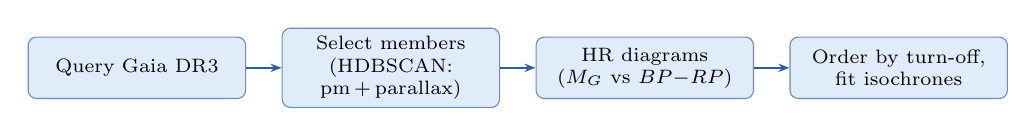
\begin{tikzpicture}[
  box/.style={draw=progborder,fill=stripbg,rounded corners=3pt,
              font=\scriptsize,text width=2.55cm,align=center,
              inner sep=3pt,minimum height=0.78cm},
  arr/.style={-{Stealth[length=4pt]},progfill,line width=0.8pt}
]
  \node[box] (q) {Query Gaia DR3};
  \node[box,right=0.45cm of q] (m) {Select members\\(HDBSCAN:\\pm\,+\,parallax)};
  \node[box,right=0.45cm of m] (h) {HR diagrams\\($M_G$ vs $BP{-}RP$)};
  \node[box,right=0.45cm of h] (o) {Order by turn-off,\\fit isochrones};
  \draw[arr] (q) -- (m);
  \draw[arr] (m) -- (h);
  \draw[arr] (h) -- (o);
\end{tikzpicture}
\end{center}

\begin{center}
  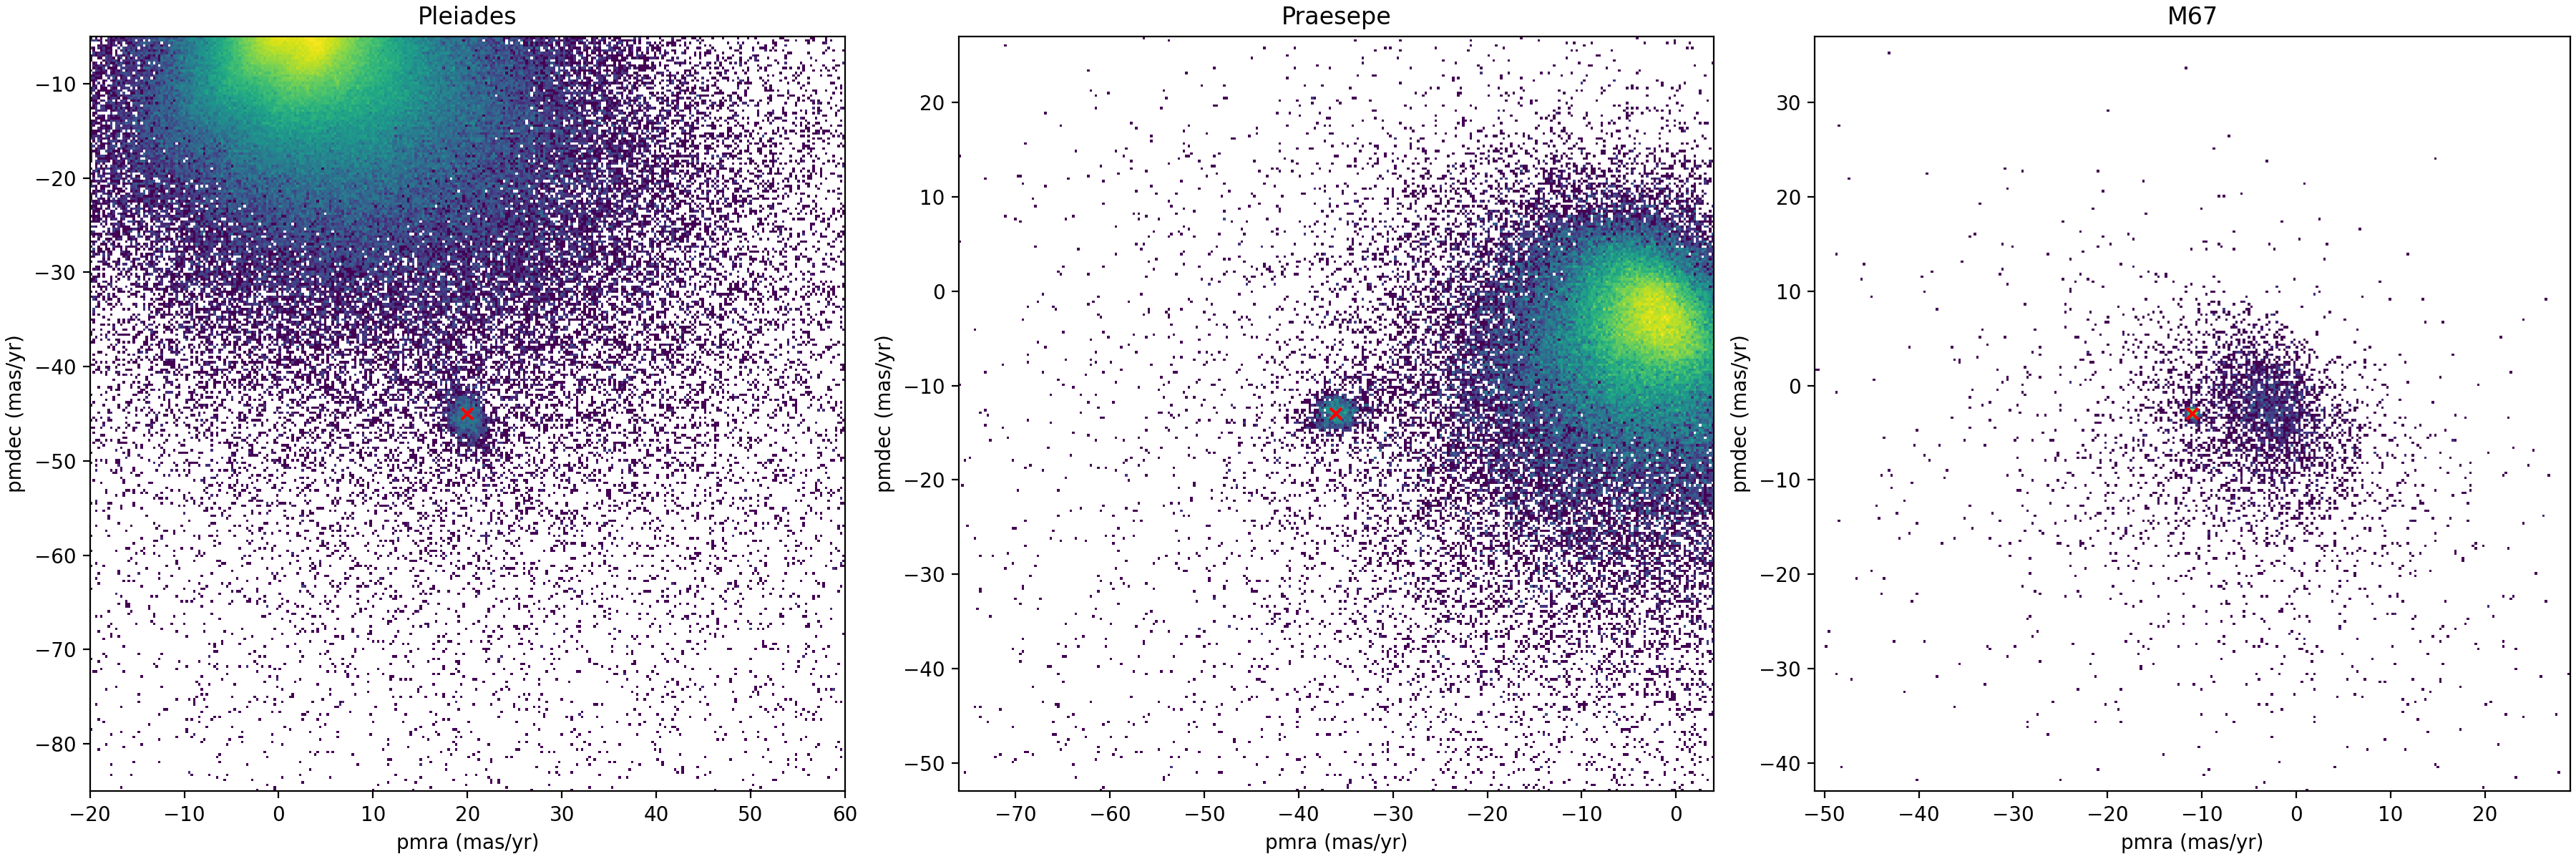
\includegraphics[width=0.85\textwidth,height=0.34\textheight,keepaspectratio]{pm_all.png}\\[-1pt]
  {\scriptsize Clusters stand out as clumps in proper motion; red cross\,=\,expected centre.}
\end{center}

{\scriptsize Working method: plan first, one stage per prompt, run and check each stage, commit.}

\vspace{2pt}
\takeaway{Answer}{Order: Pleiades $<$ Praesepe $<$ M67.
  Praesepe 709~Myr (range 654--806~Myr);
  M67 4038~Myr (range 3766--4495~Myr);
  Pleiades age not constrained (flat loss curve, no turn-off).}

\end{frame}

% ------------------------------------------------------------------
% FRAME 2 — Members and distances
% ------------------------------------------------------------------
\begin{frame}
\frametitle{Step 1: Clustering isolates each cluster at its expected distance.}
\vspace{4pt}

\methodstrip{Method}{HDBSCAN on standardised ($\mu_{\alpha^*}$, $\mu_\delta$, parallax)
  after a proper-motion pre-selection window;
  \texttt{min\_cluster\_size=50}, \texttt{min\_samples=10}
  (default settings returned only noise).}

\begin{center}
  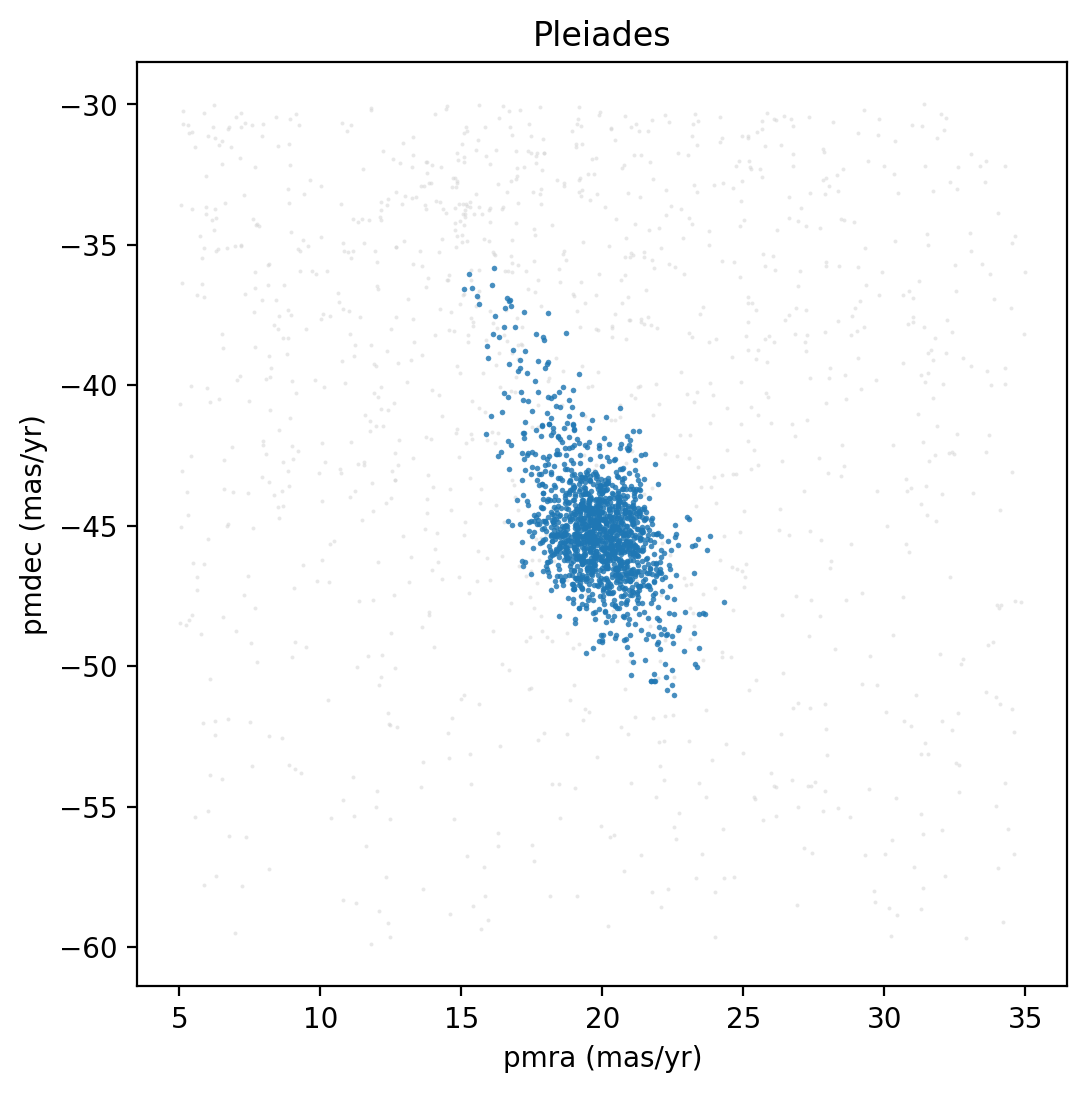
\includegraphics[width=0.292\textwidth,height=0.27\textheight,keepaspectratio]{pm_members_pleiades.png}%
  \hspace{0.009\textwidth}%
  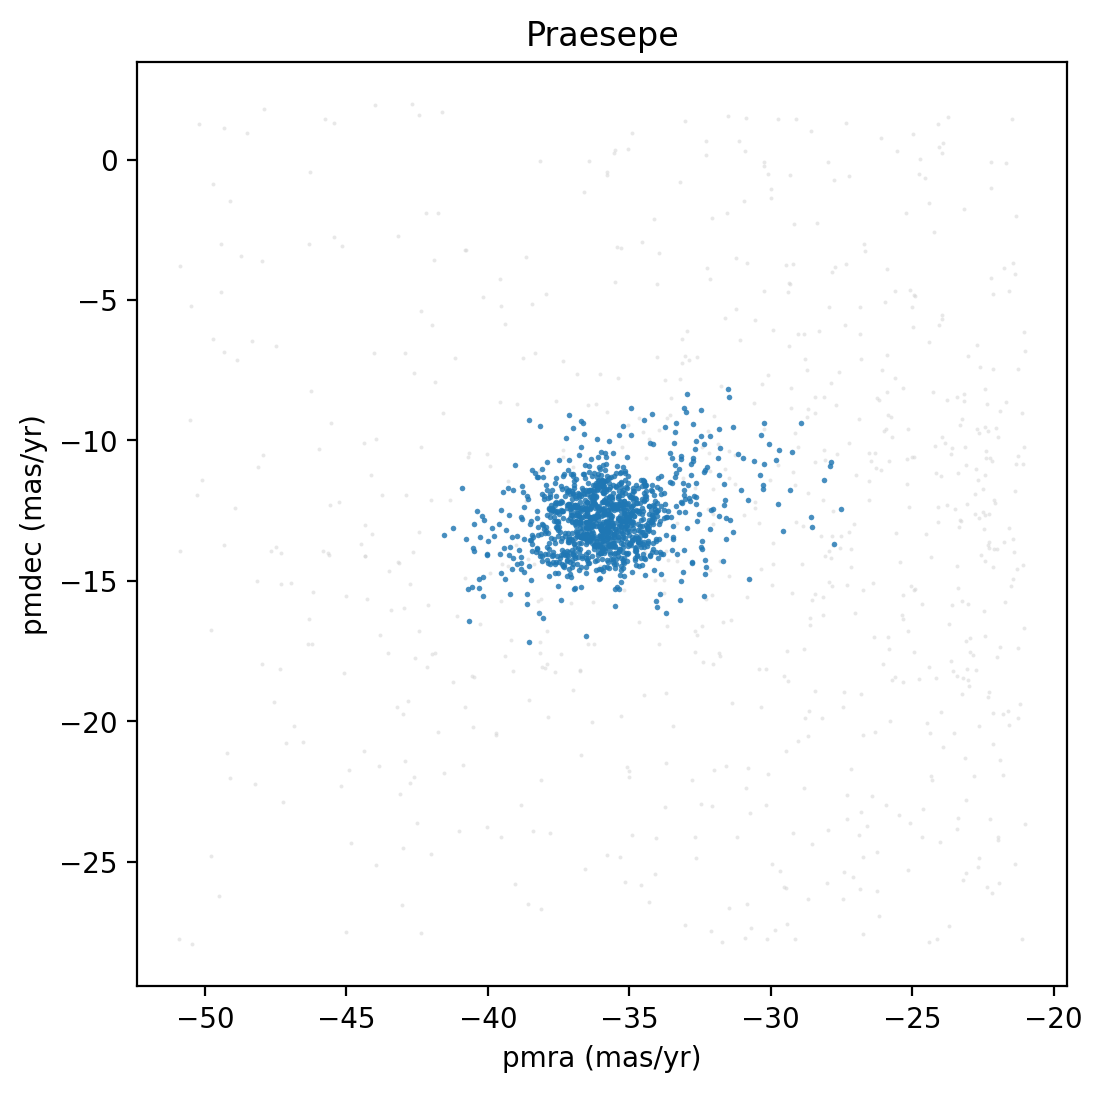
\includegraphics[width=0.292\textwidth,height=0.27\textheight,keepaspectratio]{pm_members_praesepe.png}%
  \hspace{0.009\textwidth}%
  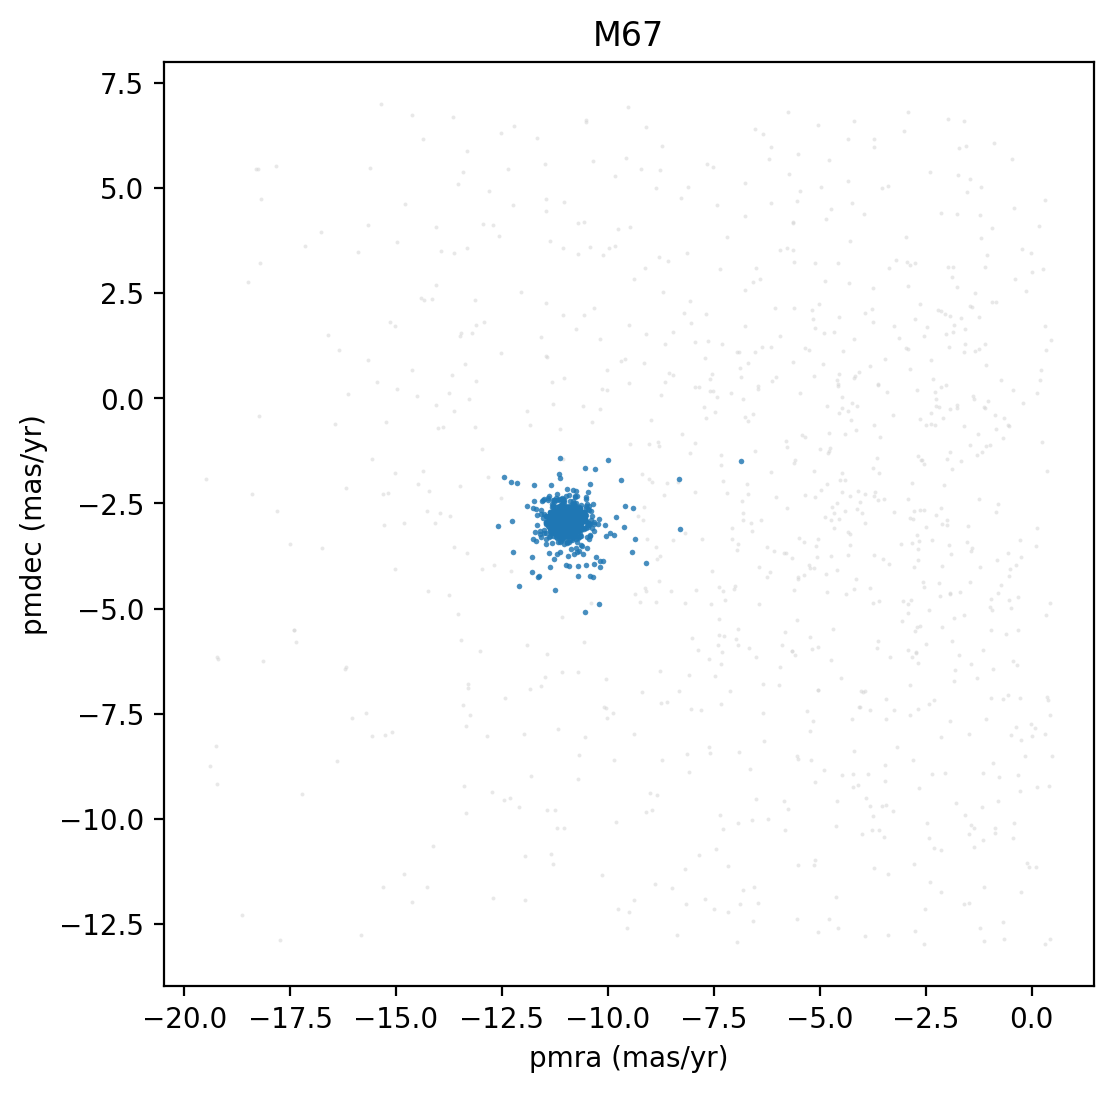
\includegraphics[width=0.292\textwidth,height=0.27\textheight,keepaspectratio]{pm_members_m67.png}
\end{center}

\vspace{-4pt}
\begin{center}
\footnotesize
\renewcommand{\arraystretch}{1.0}
\begin{tabular}{@{}>{\centering\arraybackslash}p{0.14\textwidth}>{\centering\arraybackslash}p{0.10\textwidth}>{\centering\arraybackslash}p{0.18\textwidth}>{\centering\arraybackslash}p{0.18\textwidth}>{\centering\arraybackslash}p{0.14\textwidth}@{}}
\toprule
Cluster & $N$ & $d_{\rm raw}$ (pc) & $d_{+0.017\,\rm mas}$ (pc)$^{a}$ & $d_{\rm ref}$ (pc) \\
\midrule
Pleiades & 1417 & 136.0 & 135.7 & 136.0 \\
Praesepe & 1136 & 185.0 & 184.5 & 185.0 \\
M67 & 1315 & 866.6 & 854.0 & 850.0 \\
\bottomrule
\multicolumn{5}{@{}p{0.74\textwidth}@{}}{\scriptsize
  $^{a}$Approx.\ global zero-point of $+0.017$~mas. Reference distances from \texttt{src/config.py}. The reference distances are rounded literature values, so this is a consistency check and not an independent validation of the zero-point offset.}
\end{tabular}
\end{center}

\vspace{-2pt}
\takeaway{Takeaway}{Distances agree with the references within 0.5\% (largest: M67, $+0.47\%$);\\ counts 1417 / 1136 / 1315 are somewhat above the expected few hundred to about 1000.}

\vspace{0.3cm}

\end{frame}

% ------------------------------------------------------------------
% FRAME 3 — HR diagrams
% ------------------------------------------------------------------
\begin{frame}
\frametitle{Step 2: The HR diagrams already show a sequence of evolutionary stages.}
\vspace{4pt}

\methodstrip{Method}{$M_G = G + 5\log_{10}(\varpi/100)$, $\varpi$ in mas;
  colour $BP{-}RP$; cluster members only.}

\begin{center}
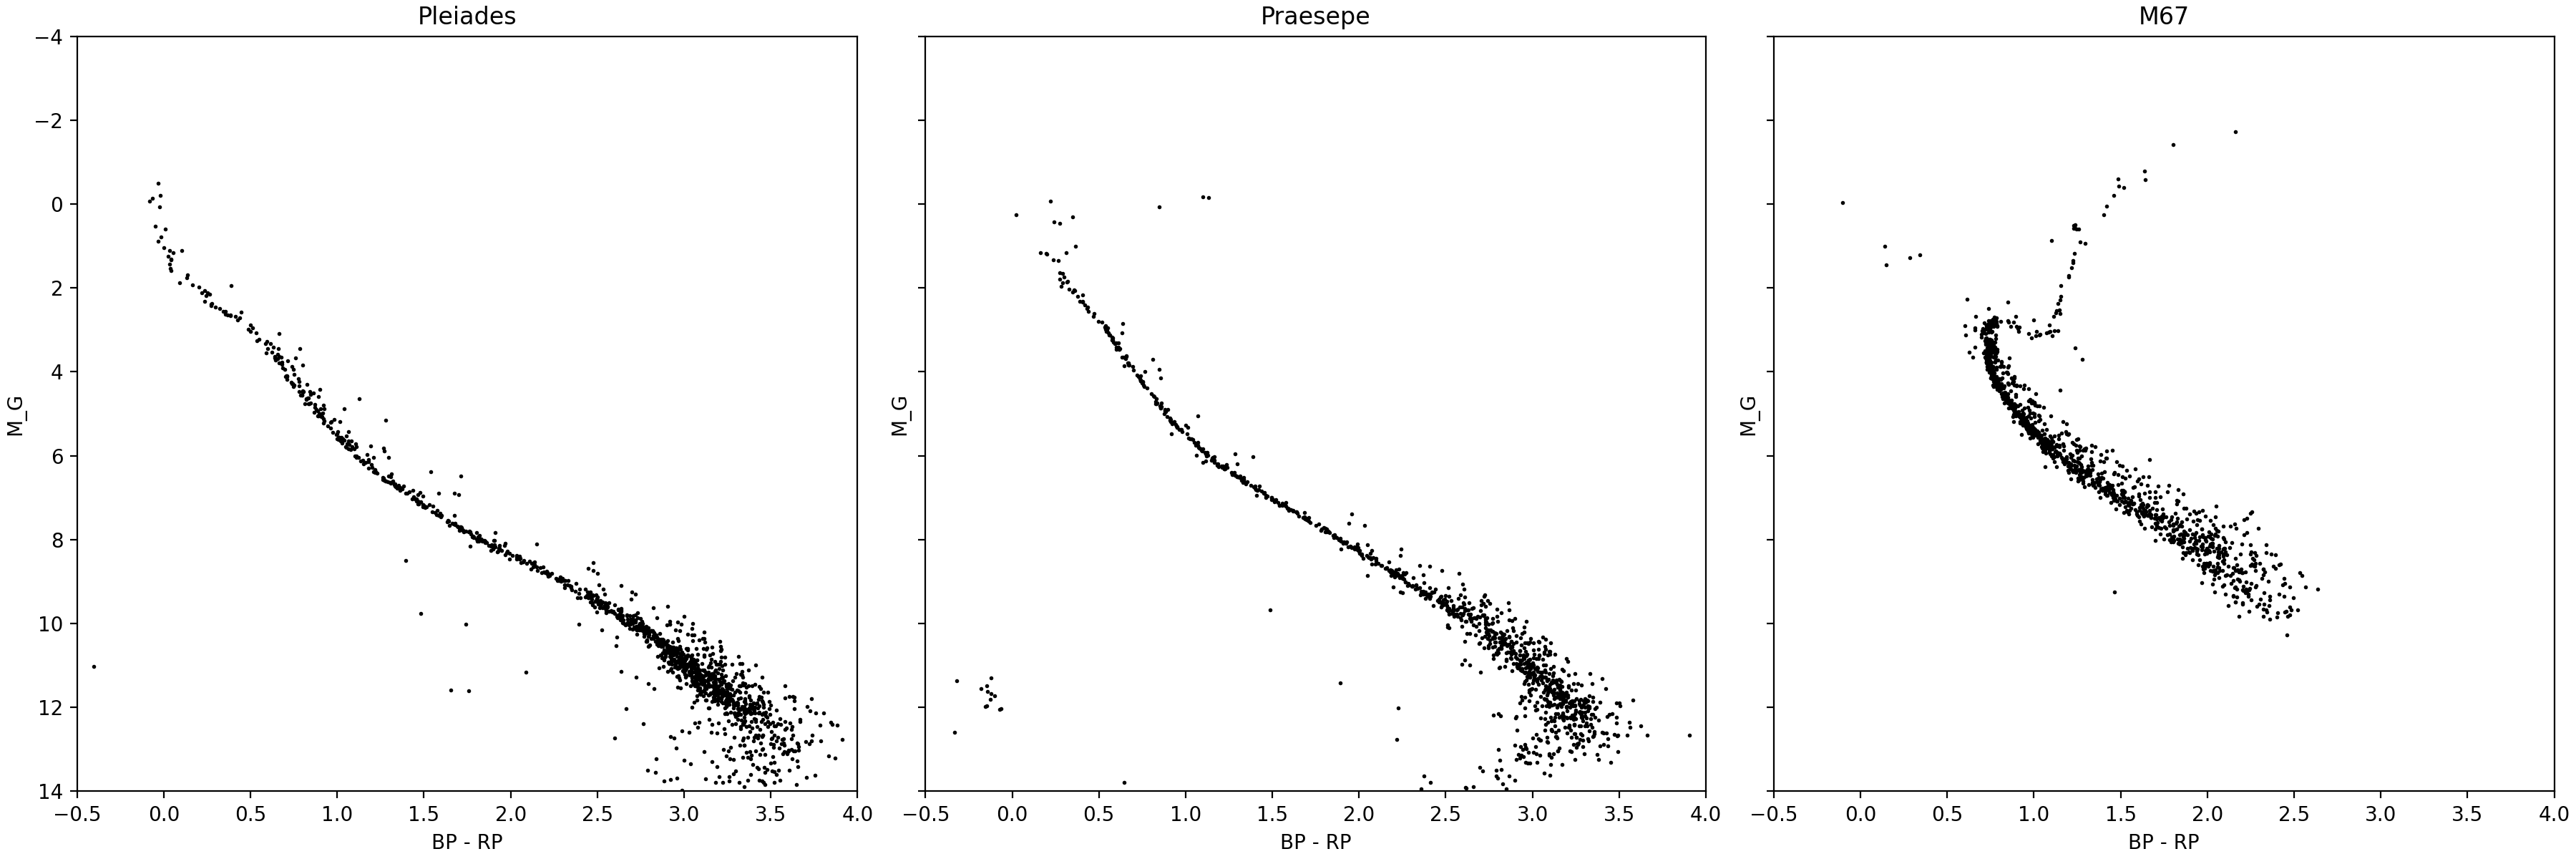
\includegraphics[width=0.89\textwidth,height=0.47\textheight,keepaspectratio]{hr_all.png}
\end{center}

\vspace{-3pt}
\begin{center}
\footnotesize
\begin{tabular}{@{}>{\raggedright\arraybackslash}p{0.29\textwidth}@{\hspace{0.01\textwidth}}%
                   >{\raggedright\arraybackslash}p{0.29\textwidth}@{\hspace{0.01\textwidth}}%
                   >{\raggedright\arraybackslash}p{0.29\textwidth}@{}}
\textbf{Pleiades:} main sequence to blue end; no evolved giants. &
\textbf{Praesepe:} red-clump giants; white-dwarf sequence at faint blue end. &
\textbf{M67:} turn-off, subgiant \& red giant branches, red clump, blue stragglers. \\
\end{tabular}
\end{center}

\vspace{-3pt}
\takeaway{Takeaway}{Evolved stars in the order
  \emph{none} (Pleiades), \emph{few} (Praesepe), \emph{many} (M67)---suggesting
  the age order before any measurement.}

\end{frame}

% ------------------------------------------------------------------
% FRAME 4 — Turn-off ordering
% ------------------------------------------------------------------
\begin{frame}
\frametitle{Step 3: The turn-off orders M67 clearly, the other two only weakly.}
\vspace{4pt}

\methodstrip{Method}{Turn-off: bluest median $BP{-}RP$ in 0.25-mag bins of $M_G$
  (${\geq}5$ stars, $-1 < M_G < 6$), 200 bootstrap resamples.
  Second measure: $M_G$ of the fifth-brightest main-sequence star.}

\begin{center}
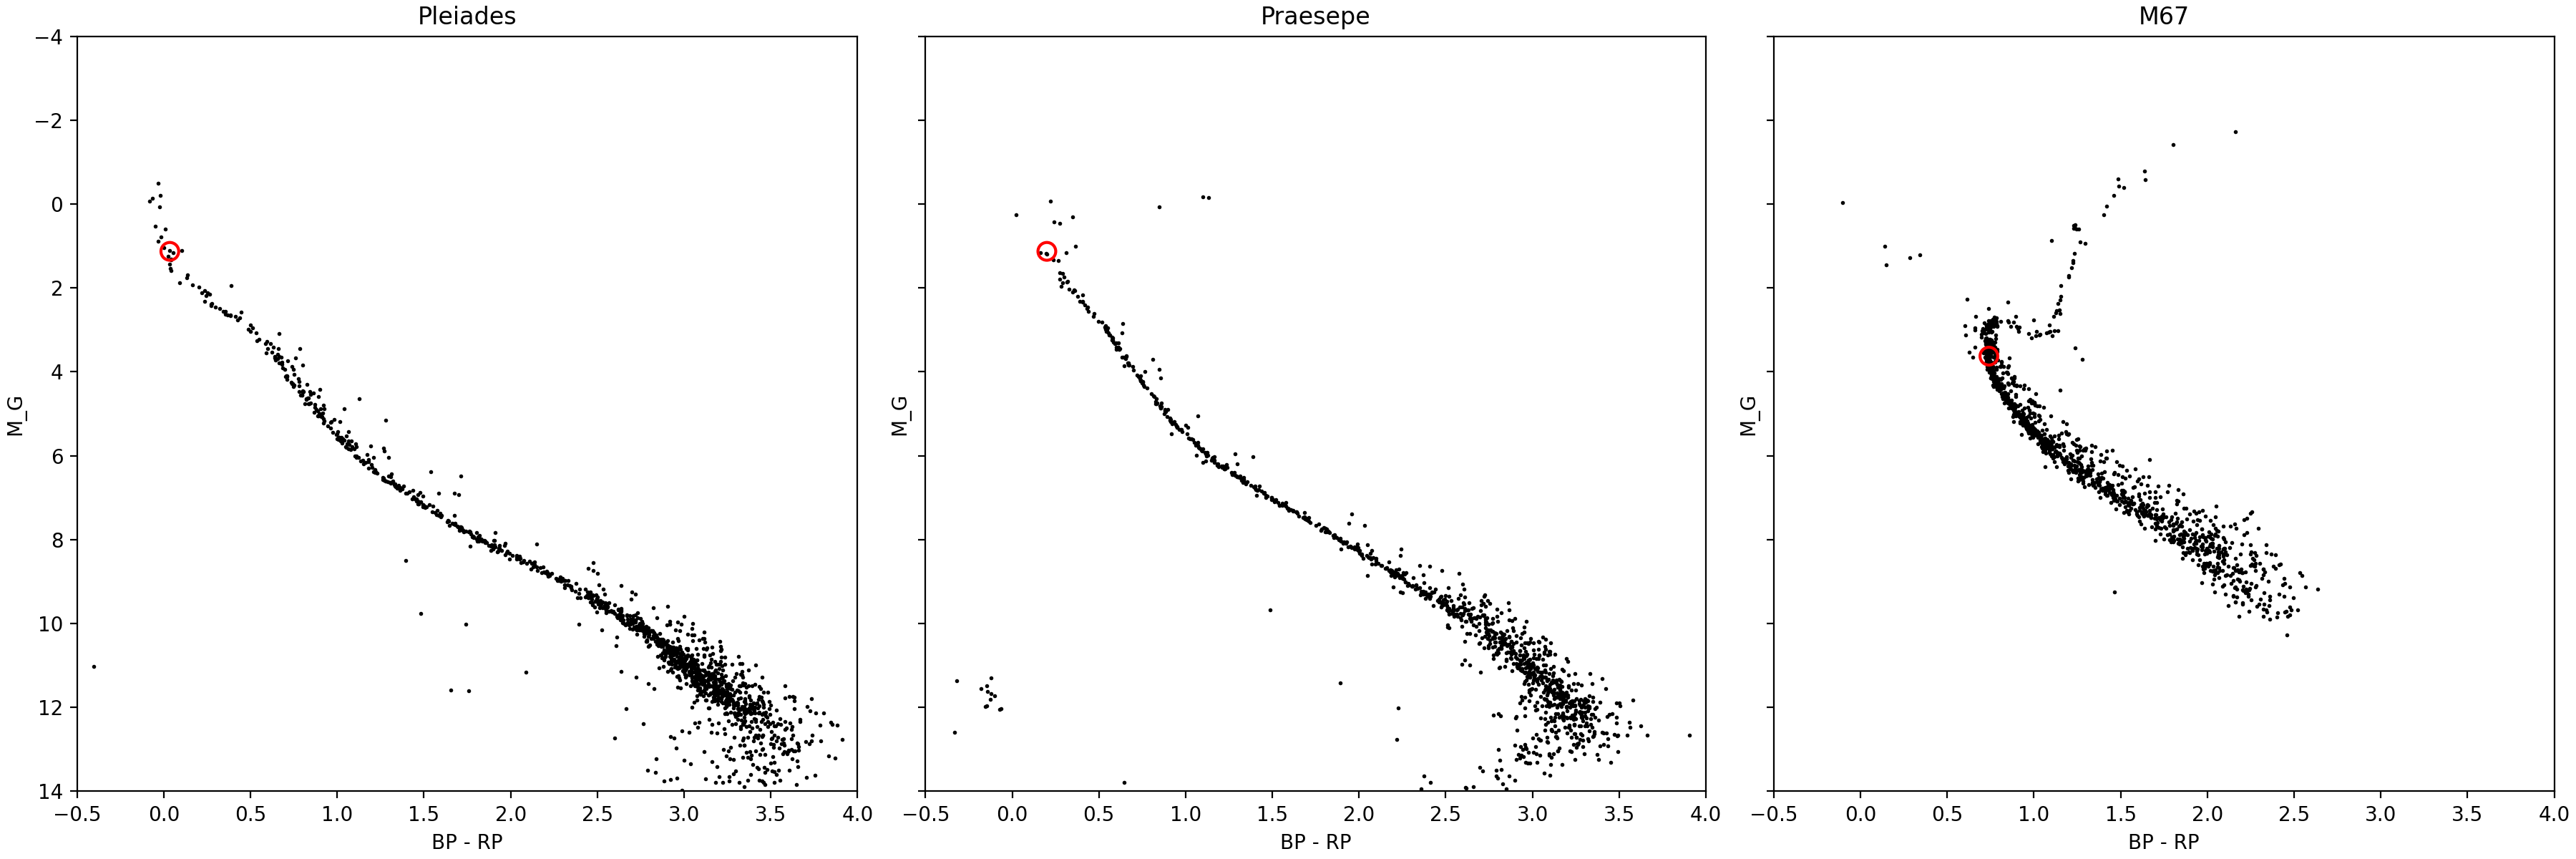
\includegraphics[width=0.88\textwidth,height=0.27\textheight,keepaspectratio]{hr_turnoff.png}
\end{center}

\vspace{-4pt}
\begin{center}
\footnotesize
\renewcommand{\arraystretch}{1.0}
\begin{tabular}{@{}>{\centering\arraybackslash}p{0.17\textwidth}>{\centering\arraybackslash}p{0.14\textwidth}>{\centering\arraybackslash}p{0.14\textwidth}>{\centering\arraybackslash}p{0.14\textwidth}>{\centering\arraybackslash}p{0.14\textwidth}@{}}
\toprule
Measure & \shortstack{Pleiades\\$<$ Praesepe} & \shortstack{Praesepe\\$<$ M67} & \shortstack{Pleiades\\$<$ M67} & \shortstack{All\\three} \\
\midrule
Colour & 0.95 & 0.875 & 0.95 & 0.83 \\
Luminosity & 0.685 & 1.0 & 1.0 & 0.685 \\
\bottomrule
\multicolumn{5}{@{}p{0.73\textwidth}@{}}{\scriptsize
  Turn-off $BP{-}RP$: Pleiades 0.035, Praesepe 0.200, M67 0.740. No clear knee for Pleiades and Praesepe. Bootstrap reflects sampling noise only.}
\end{tabular}
\end{center}

\vspace{-2pt}
\takeaway{Takeaway}{M67 is clearly oldest in luminosity (1.0 in both pairs; colour: 0.875 and 0.95).\\ Pleiades $<$ Praesepe: suggestive (colour 0.95, luminosity 0.685), not proven.}

\vspace{0.3cm}

\end{frame}

% ------------------------------------------------------------------
% FRAME 5 — Isochrone ages, conclusion, limitations
% ------------------------------------------------------------------
\begin{frame}
\frametitle{Step 4: Isochrone fits confirm the order, with stated limits.}
\vspace{4pt}

\methodstrip{Method}{MIST v1.2, Gaia EDR3 passbands; fixed distance \& $A_V$; age
  fitted to upper MS, turn-off and giants ($M_G<6.0$); robust CMD loss; measured colour offset; $v/v_{\rm crit}=0.4$.}

\begin{columns}[T]
  \begin{column}{0.46\linewidth}
    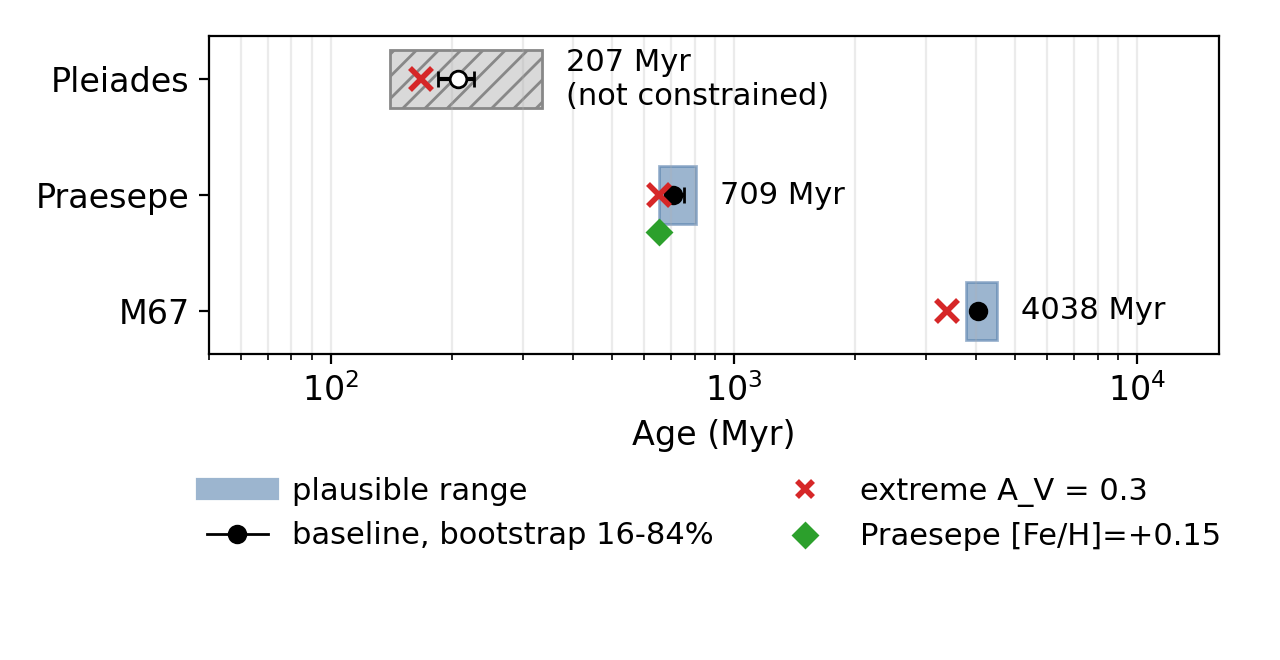
\includegraphics[width=\linewidth,height=0.18\textheight,keepaspectratio]{isochrone_summary_slide.png}\\[1pt]
    {\footnotesize\textbf{Limitations}}
    \begin{itemize}\footnotesize
      \setlength{\itemsep}{0pt}
      \setlength{\topsep}{0pt}
      \setlength{\parskip}{0pt}
      \item Colour offset 0.03--0.05 mag; reddening cannot explain it.
      \item Ranges are systematic envelopes.
      \item One model family (MIST, $v/v_{\rm crit}=0.4$); no binary modelling.
    \end{itemize}
  \end{column}
  \begin{column}{0.50\linewidth}
    \footnotesize\sloppy
    \renewcommand{\arraystretch}{1.0}
    \begin{tabular}{@{}lccc@{}}
      \toprule
      Cluster & Age & Range (Myr) & Constrained \\
      \midrule
      \rowcolor{gray!18}Pleiades & 207\,Myr & 140--334 & No$^{b}$ \\
      Praesepe & 709\,Myr & 654--806 & Yes \\
      M67 & 4038\,Myr & 3766--4495 & Yes \\
      \bottomrule
    \end{tabular}\\[1pt]
    {\scriptsize $^{b}$no: flat loss curve, no turn-off}\\[1pt]
    {\scriptsize Praesepe at [Fe/H]=+0.15: 654~Myr (approximate metallicity)}
  \end{column}
\end{columns}

{\footnotesize\textit{Context only, not a result of this analysis: literature ages about 110, 650 and 4000 Myr (Pleiades, Praesepe, M67).}}\\[1pt]
\takeaway{Takeaway}{Order Pleiades $<$ Praesepe $<$ M67; plausible ranges do not overlap.}

\end{frame}

\end{document}
